\documentclass[a4paper, 11pt]{article}           %{{{1
% basic packages                                 {{{2
\usepackage[T1]{fontenc}
\usepackage[scaled=0.975]{helvet}
\usepackage[utf8]{inputenc}
\usepackage{amsmath}
\usepackage{lastpage}
\usepackage{graphicx}
\usepackage{xcolor}
\usepackage{multicol}                                                           %
\usepackage{listings}                                                           %
\usepackage{tcolorbox}                                                          % encadrement texte
% listings                                        {{{3
\definecolor{mygreen}{rgb}{0,0.6,0}
\definecolor{mygray}{rgb}{0.5,0.5,0.5}
\definecolor{mymauve}{rgb}{0.58,0,0.82}
\definecolor{deepblue}{rgb}{0,0,0.5}
\definecolor{deepred}{rgb}{0.6,0,0}
\definecolor{deepgreen}{rgb}{0,0.5,0}
\lstset{%
%       backgroundcolor=\color{white},   % choose the background color; you must add \usepackage{color} or \usepackage{xcolor}; should come as last argument
%       basicstyle=\footnotesize,        % the size of the fonts that are used for the code
%       breakatwhitespace=false,         % sets if automatic breaks should only happen at whitespace
%       breaklines=true,                 % sets automatic line breaking
%       captionpos=b,                    % sets the caption-position to bottom
        commentstyle=\color{mygreen},    % comment style
%       deletekeywords={type},           % if you want to delete keywords from the given language
%       emph={},                         % Custom highlighting
%       emphstyle=\ttb\color{deepred}    % Custom highlighting style
%       escapeinside={\%*}{*)},          % if you want to add LaTeX within your code
%       extendedchars=true,              % lets you use non-ASCII characters; for 8-bits encodings only, does not work with UTF-8
        frame=shadowbox,                 % adds a frame around the code {single, shadowbox}
%       keepspaces=true,                 % keeps spaces in text, useful for keeping indentation of code (possibly needs columns=flexible)
        keywordstyle=\color{blue},       % keyword style
	language=C,                      % the language of the code {Python, C}
%       morekeywords={*,...},            % if you want to add more keywords to the set
        numbers=left,                    % numbers = (none, left, right)
%       numbersep=5pt,                   % how far the line-numbers are from the code
%       numberstyle=\tiny\color{mygray}, % the style that is used for the line-numbers
%       otherkeywords={self},            % Add keywords here
%       rulecolor=\color{black},         % if not set, the frame-color may be changed on line-breaks within not-black text (e.g. comments (green here))
	rulesepcolor=\color{gray}        % shadowbox color
%       showspaces=false,                % show spaces everywhere adding particular underscores; it overrides 'showstringspaces'
%       showstringspaces=false,          % underline spaces within strings only
%       showtabs=false,                  % show tabs within strings adding particular underscores
%       stepnumber=1,                    % the step between two line-numbers. If it's 1, each line will be numbered
%       stringstyle=\color{mymauve},     % string literal style
%       tabsize=4,                       % sets default tabsize to 2 spaces
%       title=\lstname                   % show the filename of files included with \lstinputlisting; also try caption instead of title
}
%}}}
%}}}
% mise en page                                   {{{2
\addtolength{\voffset}{-1.8cm}
\addtolength{\textheight}{4cm}
\addtolength{\hoffset}{-2.5cm}
\addtolength{\textwidth}{4cm}
\addtolength{\headsep}{-0.5cm}
\usepackage{fancyhdr}
\setlength{\headheight}{14.00pt}
\pagestyle{fancy} % Numérotation des pages
\renewcommand\headrulewidth{1pt}
\fancyhead[L]{BP SN}
\fancyhead[C]{arduino}
\fancyhead[R]{LED constituants des feux rouges}
\renewcommand\footrulewidth{1pt}
\fancyfoot[L]{v 1.5 -- JB}
\fancyfoot[C]{Système de contrôle d'accès : signalisation}
\fancyfoot[R]{\thepage/\pageref{LastPage}}
%\lhead{3E}%haut de page gauche
%}}}
% Compteurs:                                     {{{2
\addtocounter{page}{0}
\newcounter{Q}
\newcounter{exoNB}
%}}}
% Longueur:                                      {{{2
\newlength{\longueurA}
\newlength{\longueurB}
\setlength{\parindent}{0pt}
\setlength{\parskip}{2pt}
\renewcommand{\baselinestretch}{1}
%}}}
% newcommand                                     {{{2
\newcommand{\question}{\stepcounter{Q} $\boxed{\arabic{Q}}$ }
\newcommand{\reponse}{
\par\nobreak
\noindent\rule{0pt}{1.5\baselineskip}% Provides a larger gap between the preceding paragraph and the dots
{\noindent\makebox[\linewidth]{\dotfill}\endgraf}% ... dotted lines ...
% \bigskip% Gap between dots and next paragraph
}

\newcommand{\ligne}{\underline{\hspace{ \textwidth}} }
\newcommand{\exo}[1]{\stepcounter{exoNB}\textsc{\Large Exercice \arabic{exoNB} -- #1} }
\newcommand{\EXO}[2]{\stepcounter{exoNB}\textsc{\Large Exercice \arabic{exoNB} -- #1} \hfill \textbf{#2 points}}
\newcommand{\pb}[1] {\stepcounter{exoNB}\textsc{\Large Problème \arabic{exoNB} -- #1} }
\newcommand{\PB}[2] {\stepcounter{exoNB}\textsc{\Large Problème \arabic{exoNB} -- #1} \hfill \textbf{#2 points}}

\newcommand{\objectif}[1]{\textsc{\huge \textbf{Objectif :}\\[2mm] #1} }
\newcommand{\partie}[1]{\textsc{\LARGE #1} }
%}}}
% Divers                                         {{{2
% PRL style line                                 {{{3
\newlength{\diamondrulelength}
\setlength{\diamondrulelength}{0.6\textwidth}
\newlength{\diamondrulethickness}
\setlength{\diamondrulethickness}{2pt}
\newcommand{\diamondrule}{\begin{center}\tikz{\fill[black] (0.5\diamondrulelength,0) -- (0,0.5\diamondrulethickness) -- (-0.5\diamondrulelength,0) -- (0,-0.5\diamondrulethickness) -- cycle;}\end{center}}
%}}}
% fixed with tabular                             {{{3
\usepackage{array}
\newcolumntype{L}[1]{>{\raggedright\let\newline\\\arraybackslash\hspace{0pt}}m{#1}}
\newcolumntype{C}[1]{>{\centering\let\newline\\\arraybackslash\hspace{0pt}}m{#1}}
\newcolumntype{R}[1]{>{\raggedleft\let\newline\\\arraybackslash\hspace{0pt}}m{#1}}
%}}}
%}}}
%}}}


% http://wiki.keyestudio.com/index.php/Ks0080(81,_82)keyestudio_Maker_Learning_Kit_for_Arduino#Project_5:_Traffic_Light

\begin{document}
\sffamily
\hfill Nom : {\noindent\makebox[5cm]{\dotfill}\endgraf}
\objectif{Séquencement et controle du temps}\\

Ce système va vous apprendre à gérer des séquences d'instruction, le contrôle du temps et de bouton à l'aide d'un microcontrolleur. Ultimement, il simule les deux feux rouges situés à une intersection.

\bigskip


\partie{Materiel}                         %{{{1
\begin{multicols}{2}
- Arduino board *1\\
- USB cable *1\\
- Red M5 LED*2\\
- Yellow M5 LED*2\\
- Green M5 LED*2\\
- 220$\Omega$ resistor *6\\
- Breadboard*1\\
\end{multicols}
%\begin{figure}[h!]
%\begin{center}
%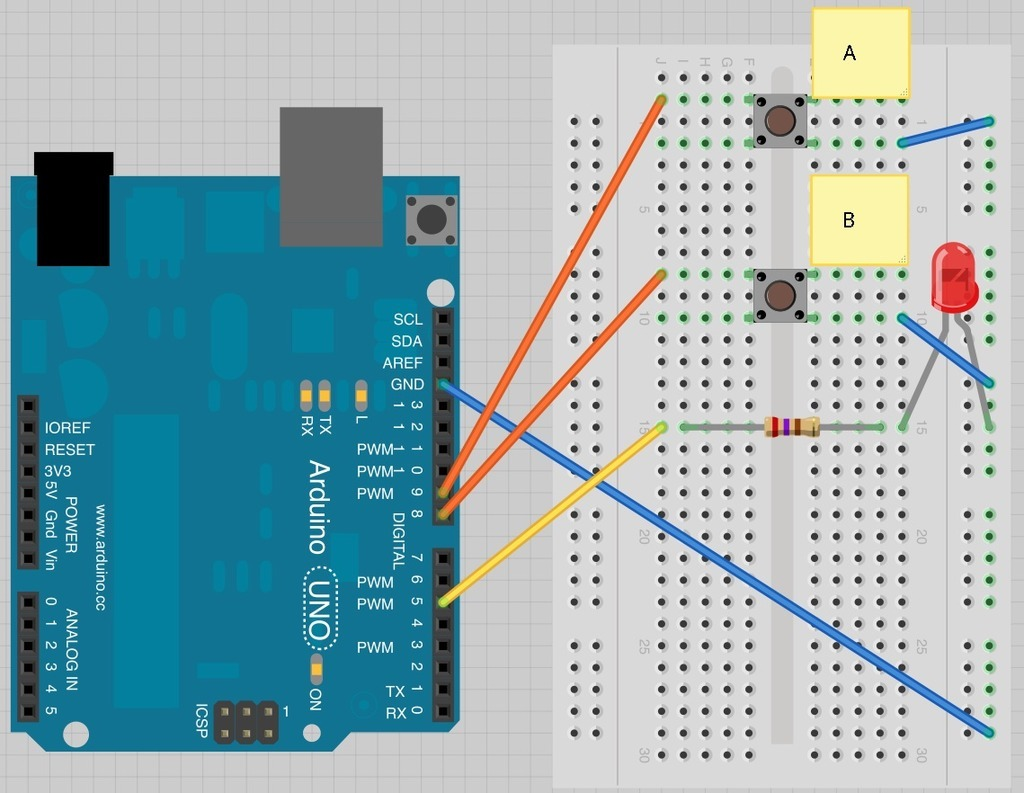
\includegraphics[width=0.75\textwidth]{cablage}
%\caption{Cablage des deux feux rouges : montage final du sujet.}
%\end{center}
%\end{figure}
%}}}


\bigskip


\partie{Un seul feu rouge}\\             %{{{1
D'abord, prennez en main le cablage des LED et leur programmation avec le microcontrolleur en faisant fonctionner le montage de la figure \ref{UnFeuRouge}.

\begin{figure}[!b]
\begin{center}
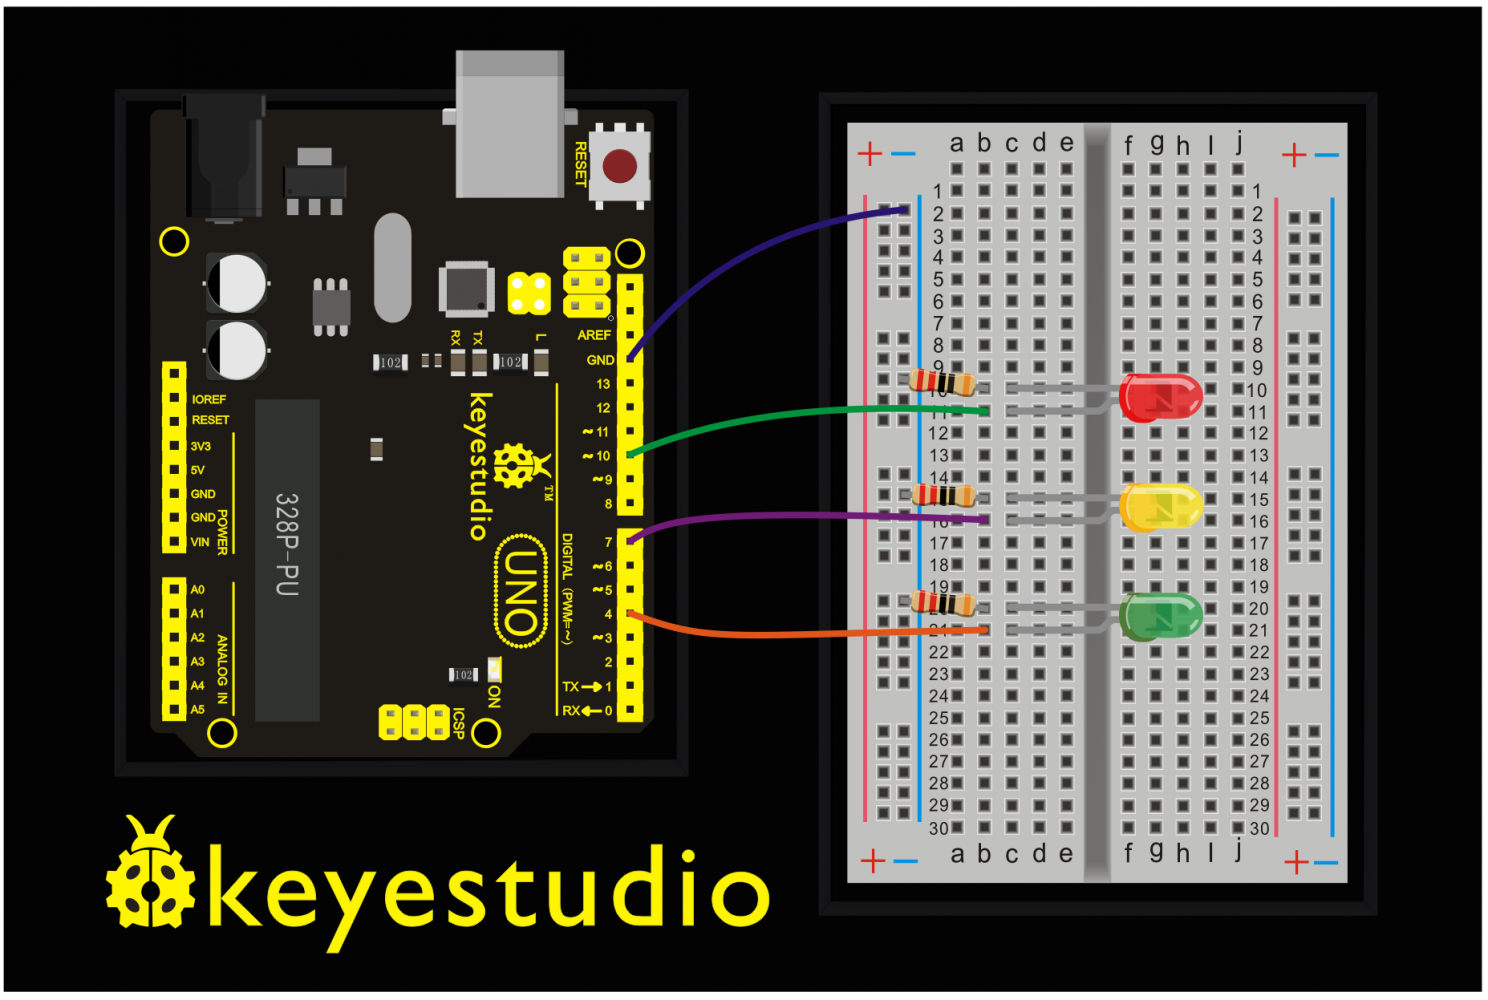
\includegraphics[width=\textwidth]{UnFeuRouge}
\caption{Cablage d'un seul feu rouge}
\label{UnFeuRouge}
\end{center}
\end{figure}

\question Quel courant faut-il dans chaque LED ?
\reponse
\reponse
\reponse



\question Quel tension chute aux bornes des trois LED ?
\reponse
\reponse
\reponse

\question En déduire la valeur de chaque résistance en série avec les LED ?
\reponse
\reponse
\reponse

\question Quelles résistances $R_R, R_V, R_J$ du matériel prennons-nous effectivement ?
\reponse

\question Impémenter le code suivant et résumer d'une phrase le comportement observé.
\reponse
\begin{lstlisting}
int redled =10;                		// initialize digital pin 10
int yellowled =7;              		// initialize digital pin 7
int greenled =4;               		// initialize digital pin 4
void setup() {
	pinMode(redled, OUTPUT);        // pin with red LED as output
	pinMode(yellowled, OUTPUT);     // pin with yellow LED as output
	pinMode(greenled, OUTPUT);      // pin with green LED as output
}
void loop()
	{
	digitalWrite(greenled, HIGH);  		// turn on green LED
	delay(5000);                   		// wait 5 seconds
	digitalWrite(greenled, LOW);   		// turn off green LED
	for(int i=0;i<3;i++) {         		// blinks for 3 times
		delay(500);                     // wait 0.5 second
		digitalWrite(yellowled, HIGH);  // turn on yellow LED
		delay(500);                     // wait 0.5 second
		digitalWrite(yellowled, LOW);   // turn off yellow LED
	}
	delay(500);                    		// wait 0.5 second
	digitalWrite(redled, HIGH);    		// turn on red LED
	delay(5000);                   		// wait 5 second
	digitalWrite(redled, LOW);     		// turn off red LED
}
\end{lstlisting}

\tcbox{\textbf{Constatation professeur :} \hspace{5cm} } % package tcolorbox

\question Décrire l'algorithme quasiment ligne à ligne.
\reponse
\reponse
\reponse
\reponse
\reponse
\reponse

%}}}


\bigskip


\partie{Un seul feu rouge et un bouton}\\ %{{{1
%\begin{center}
%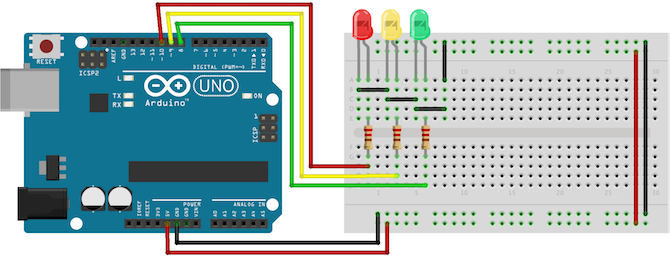
\includegraphics[width=0.5\textwidth]{Arduino_Traffic_Light}
%\end{center}


\question Programmer un simple feu rouge avec un bouton.
\begin{figure}[h]
\begin{center}
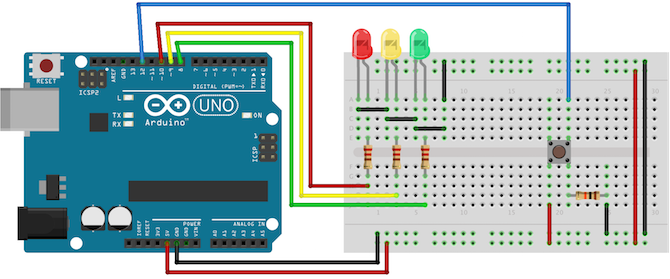
\includegraphics[width=\textwidth]{Arduino_Traffic_Light_With_Button}
\caption{Feu de signalisation avec un bouton}
\end{center}
\end{figure}

\begin{lstlisting}
int red = 10;
int yellow = 9;
int green = 8;
int button = 12;

void setup(){
    pinMode(red, OUTPUT);
    pinMode(yellow, OUTPUT);
    pinMode(green, OUTPUT);
    pinMode(button, INPUT);
    digitalWrite(green, HIGH);
}

void loop() {
    if (digitalRead(button) == HIGH){
        delay(15); // software debounce
        if (digitalRead(button) == HIGH) {
            changeLights();
            delay(15000); // wait for 15 seconds
        }
    }
}

void changeLights(){
    digitalWrite(green, LOW);
    digitalWrite(yellow, HIGH);
    delay(3000);

    digitalWrite(yellow, LOW);
    digitalWrite(red, HIGH);
    delay(5000);

    digitalWrite(red, LOW);
    digitalWrite(green, HIGH);
    delay(3000);
}

\end{lstlisting}

\tcbox{\textbf{Constatation professeur :} \hspace{5cm} } % package tcolorbox

\question A la fin de la fonction \texttt{setup()}, dans quels états sont les DEL verte, rouge et orange ?
\reponse

\question Combien de temps doit rester appuyé le bouton pour permettre l'instruction à la ligne 18 ?
\reponse

\question Que fait l'instruction de la ligne 18 ?
\reponse

\question Combien de temps restent allumées les lumières orange et rouge avant de changer ?
\reponse

\question A la ligne 16, il y a écrit \texttt{software debounce}. Pourquoi software ? Pouquoi debounce ?
\reponse
\reponse

\question Quelle valeur retourne la fonction changeLights() ?
\reponse

%}}}


\bigskip


\partie{Deux feux rouges}\\               %{{{1

\begin{figure}[h]
\begin{center}
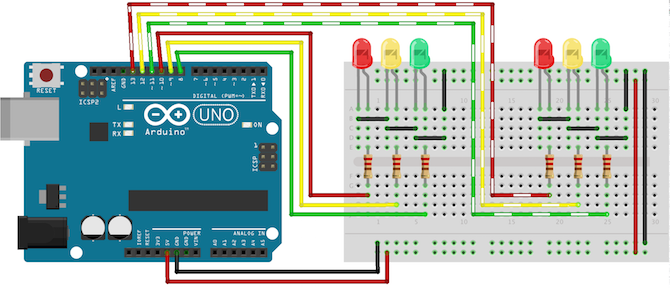
\includegraphics[width=\textwidth]{Arduino_Dual_Traffic_light}
\caption{Cablage de deux feux rouges à une intersection}
\label{cablage2feux}
\end{center}
\end{figure}
%
\question Pour l'exercice, implémentons des feux de croisement avec le séquencement qu'ils ont aux états-unis. Ce séquencement est précisé dans la figure \ref{sequenceUSA}. Décrire ce qui change par rapport aux feux rouges français.
\reponse
\begin{figure}[h]
\begin{center}
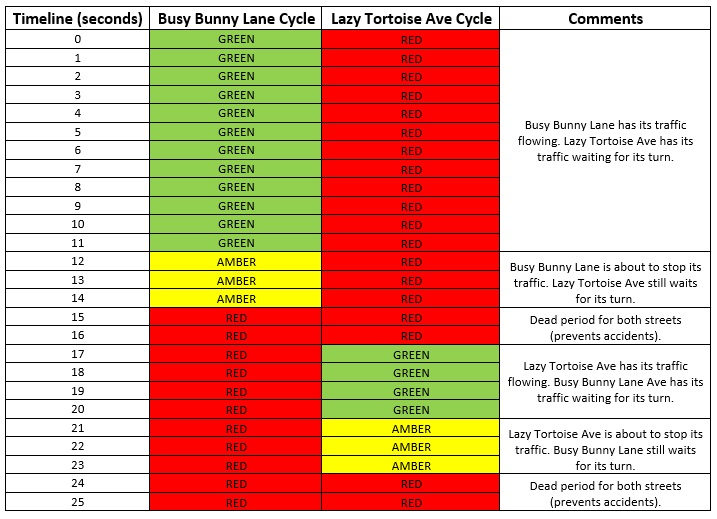
\includegraphics[width=\textwidth]{trafficchartUSAJPG}
\caption{sequencement des feux rouges aux états-unis. }
\label{sequenceUSA}
\end{center}
\end{figure}
%
\question Implémenter ce code et le cablage de la figure \ref{cablage2feux}.

\begin{lstlisting}
int red1 = 10;
int yellow1 = 9;
int green1 = 8;
int red2 = 13;
int yellow2 = 12;
int green2 = 11;

void setup(){
    pinMode(red1, OUTPUT);
    pinMode(yellow1, OUTPUT);
    pinMode(green1, OUTPUT);

    pinMode(red2, OUTPUT);
    pinMode(yellow2, OUTPUT);
    pinMode(green2, OUTPUT);
}

void loop(){
    changeLights();
    delay(15000);
}

void changeLights(){
    // turn both yellows on
    digitalWrite(green1, LOW);
    digitalWrite(yellow1, HIGH);
    digitalWrite(yellow2, HIGH);
    delay(5000);

    // turn both yellows off, and opposite green and red
    digitalWrite(yellow1, LOW);
    digitalWrite(red1, HIGH);
    digitalWrite(yellow2, LOW);
    digitalWrite(red2, LOW);
    digitalWrite(green2, HIGH);
    delay(5000);

    // both yellows on again
    digitalWrite(yellow1, HIGH);
    digitalWrite(yellow2, HIGH);
    digitalWrite(green2, LOW);
    delay(3000);

    // turn both yellows off, and opposite green and red
    digitalWrite(green1, HIGH);
    digitalWrite(yellow1, LOW);
    digitalWrite(red1, LOW);
    digitalWrite(yellow2, LOW);
    digitalWrite(red2, HIGH);
    delay(5000);
}
\end{lstlisting}

\tcbox{\textbf{Constatation professeur :} \hspace{5cm} } % package tcolorbox

%}}}


\end{document}

